
\note{Need to update numbers and mention how only fluxes with SNR $>20$ and galaxies with at least 4 fluxes were kept. Also, I removed FUV because it's not broadband.}
Our data set consists of 111,797 galaxies with redshifts $z < 4.54$ and $i$-band magnitudes in the range $13.8 < i < 27.4$. 
This set is divided into a training set, from which SED templates are learned, and a test set, for which photo-z's are estimated using the learned templates. 
The redshift surveys in each set are distinct, but there is overlap in the broadband filters used to measure the photometry.
The entire data set is summarized in Table \ref{tab:data_sets}, the filters used to measure photometry are listed in Table \ref{tab:filters}, and the redshift distributions are shown in Figure \ref{fig:redshift_dist}.
The filter transmission were obtained from the Spanish Virtual Observatory (SVO) Filter Profile Service.

\begin{table*}
    \centering
    \caption{Summary of the redshift and photometric data sets. $N_\text{gal}$ is the total number of galaxies in the set, $f_\text{gal}$ is the fraction of galaxies in the set, and $\Bar{\sigma}_i$ is the mean fractional flux error for the $i$-band photometry. \note{NOTE: Need to update this after imposing
    SNR $> 20$.}}
    \begin{tabular}{l r c c c c c c l}
        \hline \hline
        Data Set & $N_\text{gal}$ & $f_\text{gal}$ & $z_\text{mean}$ & $z_\text{max}$ & $i$-band range & $i_\text{mean}$ & $\Bar{\sigma}_i$ & Reference \\
        \hline
        
        zCOSMOS  &  14311 & 0.13 & 0.57 & 2.52 & $16.87 \leq i \leq 24.29$ & 21.19 & 0.06 & \citet{Lilly2009a} \\
        VVDS     &   9665 & 0.09 & 0.64 & 4.54 & $13.84 \leq i \leq 26.75$ & 20.95 & 0.03 & \citet{LeFevre2013b} \\
        VIPERS   &  71951 & 0.64 & 0.70 & 2.15 & $17.66 \leq i \leq 23.25$ & 21.41 & 0.02 & \citet{Scodeggio2018a} \\
        DEEP2/3  &  14029 & 0.13 & 0.73 & 1.98 & $15.30 \leq i \leq 25.36$ & 21.57 & 0.04 & \citet{Zhou2019a,Newman2013b} \\
        3D-HST   &   1621 & 0.01 & 1.50 & 3.32 & $19.10 \leq i \leq 27.41$ & 23.83 & 0.04 & \citet{Zhou2019a,Momcheva2016b}\\
        \hline
        Training &  89261 & 0.80 & 0.70 & 4.54 & $13.84 \leq i \leq 26.75$ & 27.41 & 0.03 \\
        Test     &  22316 & 0.20 & 0.69 & 3.74 & $16.46 \leq i \leq 27.41$ & 26.78 & 0.03 \\
        \hline
        Total    & 111577 & 1.00 & 0.70 & 4.54 & $13.84 \leq i \leq 27.41$ & 21.36 & 0.03 \\
        
        \hline
    \end{tabular}
    \label{tab:data_sets}
\end{table*}

\subsection{Training Set}

The training set is the set of galaxies from which the SED templates are learned, according to the methods described in Section \ref{sect:template_training}.
It consists of 95,927 galaxies ($86\%$ of all galaxies) with redshifts $z < 4.54$ and $i$-band magnitudes in the range $13.8 < i < 26.8$.
The training set is composed of three spec-z surveys, zCOSMOS-\textit{bright} \citep{Lilly2009a}, VVDS \citep{LeFevre2013b}, and VIPERS \citep{Scodeggio2018a}, each conducted with the VIMOS spectrograph mounted on the European Southern Observatory's (ESO) Very Large Telescope (VLT).
The spec-z's are matched to broadband photometry from the GALEX, CFHT (Megacam and CFH12k), Subaru, and UKIRT telescopes (see Table \ref{tab:filters}).
\note{Cite Martin when I cite GALEX}.

\begin{table}
    \centering
    \caption{The 19 filters used to measure the galaxy photometry in the data set. Mean wavelength, $\lambda_0 = \int \lambda R(\lambda) d\lambda$, and effective width, $W_\text{eff} = \text{Max}[R(\lambda)]^{-1}$, are given in angstroms. Filters are listed in order of increasing $\lambda_0$.}
    \begin{tabular}{l c c r r}
        \hline \hline
        Filter & Telescope & Instrument & $\lambda_0$ & $W_\text{eff}$ \\
        \hline
        
        $NUV$ & GALEX  &         &  2343.1 &  767.3 \\
        $u$   & CFHT   & Megacam &  3817.7 &  525.4 \\
        $B$   & CFHT   & CFH12k  &  4342.5 &  873.6 \\
        $B_J$ & Subaru & Suprime &  4478.4 &  763.9 \\
        $g^+$ & Subaru & Suprime &  4808.5 & 1043.1 \\
        $g$   & CHFT   & Megacam &  4899.9 & 1293.8 \\
        $V$   & CFHT   & CFH12k  &  5393.7 &  882.7 \\
        $V_J$ & Subaru & Suprime &  5493.0 &  862.4 \\
        $r$   & CHFT   & Megacam &  6278.2 & 1120.2 \\
        $r^+$ & Subaru & Suprime &  6314.8 & 1211.4 \\
        $R$   & CFHT   & CFH12k  &  6603.5 & 1138.5 \\
        $i_2$ & CHFT   & Megacam &  7584.5 & 1409.4 \\
        $i$   & CHFT   & Megacam &  7676.6 & 1307.6 \\
        $i^+$ & Subaru & Suprime &  7709.1 & 1361.7 \\
        $I$   & CFHT   & CFH12k  &  8277.3 & 1816.7 \\
        $z$   & CHFT   & Megacam &  8857.6 & 1040.1 \\
        $z^+$ & Subaru & Suprime &  9054.5 & 1012.3 \\
        $Y$   & Subaru & Suprime & 10216.0 &  996.2 \\
        $J$   & UKIRT  & WFCAM   & 12508.5 & 1476.8 \\
        
        \hline
    \end{tabular}
    \label{tab:filters}
\end{table}

\subsubsection{zCOSMOS-\textit{bright}}

zCOSMOS \citep{Lilly2009a} is a redshift survey of 1.7 $\text{deg}^2$ of the COSMOS field, divided into two parts, \textit{bright} and \textit{deep}. 
We make use of the former, consisting of approximately 20,000 galaxies with redshifts $z < 1.2$.
We only use galaxies in the recommended sample described in the ESO data release description\footnote{\url{https://www.eso.org/sci/observing/phase3/data_releases/zcosmos_dr3_b2.pdf}}, determined to have $99\%$ spectroscopic verification (i.e. \texttt{zflag} = 3.x, 4.x, 2.5, 2.4, 1.5, 9.5, 9.3, 18.5, 18.3).

The zCOSMOS redshifts are matched to broadband photometry from \citet{Ilbert2009}.
The photometry is measured from the ultraviolent to the near-infrared in 12 broadband filters: $FUV$ and $NUV$ on GALEX, $u$ and $i$ on CFHT using Megacam, $B$ and $V$ on CFHT using CFH12k, $g^+$, $r^+$, $i^+$, and $z^+$ on Subaru, and $J$ on UKIRT (details in Table \ref{tab:filters}).
We use only galaxies that were not masked in any of the optical bands.
The final set consists of 14,311 galaxies with redshifts $z < 2.52$ and $i$-band magnitudes in the range $16.9 < i < 24.3$.

\subsubsection{VVDS}

The VIMOS VLT Deep Survey (VVDS, \citealt{LeFevre2013b}) is a redshift survey consisting of three component surveys: \textit{Wide}, \textit{Deep}, and \textit{Ultra-Deep}. 
The Wide survey covers 8.7 $\text{deg}^2$, with approximately 25,000 galaxies in the range $17.5 < i < 22.5$; the Deep survey covers 0.74 $\text{deg}^2$, with approximately 11,000 galaxies in the range $17.5 < i < 24$; the Ultra-Deep survey covers 512 $\text{arcmin}^2$, with approximately 900 galaxies in the range $23 < i < 24.75$.
We use redshifts with quality flags 3 and 4, indicating a 98\% spec-z confidence.
Photometry was obtained in the $u,g,r,i,z$ and $B,V,R,I$ bands from CFHT. See Table \ref{tab:filters} for details.
The final set contains 9,665 galaxies out to redshifts $z < 4.5$, with magnitudes $ 13.8 < i < 20.9$.
\note{Cite CFH12K camera at CFHT photometry from LeFevre 2004 and McCracken}.

\subsubsection{VIPERS}

The VIMOS Public Extragalactic Redshift Survey (VIPERS, \citealt{Scodeggio2018a}) is a dense, large-volume redshift survey, focusing on redshifts $0.5 < z < 1.2$. 
The survey includes 76,552 galaxies with redshifts reliable at a 95\% confidence level.
We keep only galaxies with \texttt{photoMask} and \texttt{spectroMask} = 1.
The final set contains 71,951 galaxies with redshifts $< 2.15$ and magnitudes $17.7 < i < 23.3$. 
VIPERS photometry are measured in $FUV$ and $NUV$ on GALEX, and $u,g,r,i2,i,z$ on CFHT Megacam. 
Note that $i_2$ is the replacement $i$-band filter on Megacam. 

\subsection{Test Set}

The test set is the set of galaxies for which photo-z's are estimated with \bpz, as described in Section \ref{sect:bpz}, using the SED templates learned from the training set. 
It consists of 15,650 galaxies ($14\%$ of all galaxies) with redshifts $z < 3.32$ and $i$-band magnitudes in the range $15.3 < i < 27.4$
The test set is composed of broadband photometry and spec-z's from the DEEP2/3 and 3D-HST surveys compiled in \citet{Zhou2019a}.

Paragraph about the Zhou stuff. \citep{Zhou2019a,Newman2013b,Momcheva2016b}.
\note{Need to write this.}

\begin{figure}
    \centering
    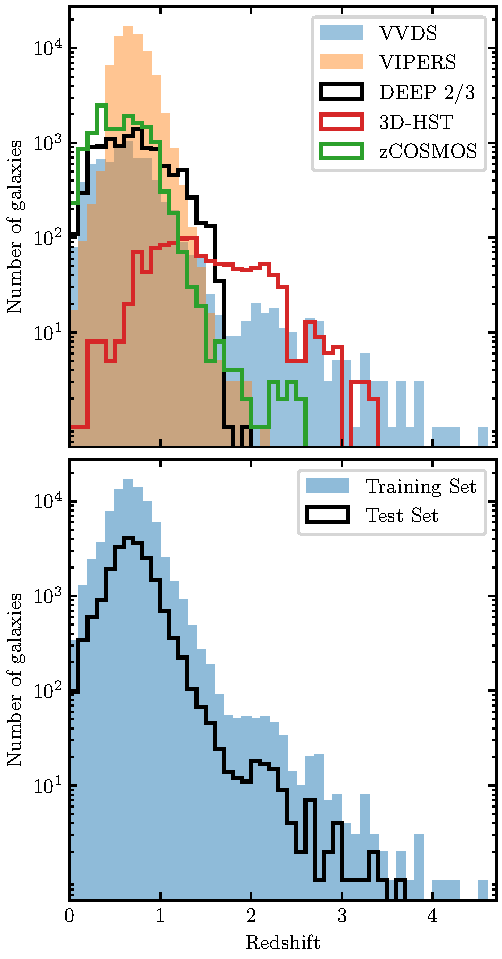
\includegraphics{figures/redshift_distribution.pdf}
    \caption{Redshift distribution of the galaxy surveys. The top and bottom panels show the redshifts of the training and test sets respectively, including the constituent surveys.}
    \label{fig:redshift_dist}
\end{figure}

